% ============================================================
% LaTeX 前置
% ============================================================
\documentclass[conference]{IEEEtran}
\usepackage{cite}
\usepackage{amsmath,amssymb,amsfonts}
\usepackage{algorithmic}
\usepackage{graphicx}
\usepackage{textcomp}
\usepackage{xcolor}
\usepackage{booktabs}
\usepackage{array}
\usepackage{multirow}
\usepackage{hyperref}

\def\BibTeX{{\rm B\kern-.05em{\sc i\kern-.025em b}\kern-.08em
    T\kern-.1667em\lower.7ex\hbox{E}\kern-.125emX}}

\begin{document}

% ============================================================
\title{Semantic-Aware Time-Sensitive Networking Scheduling with Constrained Safe Reinforcement Learning}
% ============================================================

\author{
\IEEEauthorblockN{Haichao Hu}
\IEEEauthorblockA{
\textit{Independent Researcher at Comm-AI.tech}\\
Chengdu, China\\
haichao.hu@comm-ai.tech}
}

\maketitle

% ============================================================
\begin{abstract}
% ============================================================

Time-Sensitive Networking (TSN) provides deterministic communication guarantees for industrial automation through mechanisms such as IEEE~802.1Qbv time-aware shaping and frame preemption. However, existing TSN scheduling methods optimize exclusively for network-layer metrics---throughput, jitter, end-to-end latency---ignoring the task-level semantics of industrial agents. In a multi-agent factory, the same sensor stream may tolerate 10~ms latency during routine inspection but require sub-millisecond delivery when gating an emergency stop. This semantic gap causes a fundamental misalignment between network resource allocation and application-criticality.

We present the first semantic-aware TSN scheduling framework that bridges this gap through three integrated components. First, a task intent ontology maps six industrial task types (inspection, collaboration, emergency stop, periodic control, telemetry, reconfiguration) across four criticality levels (L0--L3) to flow semantic descriptors---priority weights, urgency functions, and delayable boundaries---which are then translated to GCL and CBS parameters. Second, a Constrained Safe Reinforcement Learning (CSRL) scheduler, formulated as a Lagrangian-constrained MDP, optimizes a semantic-weighted task completion rate while treating Network Calculus (NC) worst-case delay bounds as a learnable constraint. Third, an NC safety shield validates every scheduling action against deterministic schedulability constraints before execution, providing policy-independent safety with per-criticality tolerance policies.

Evaluated on a 3-switch line topology with a 10\,ms hyperperiod under three experiment modes---static benchmark (5/8/12 flows), dynamic flow arrival (5 base + 3 arriving), and component ablation---the CSRL scheduler achieves 100\% task completion at 5 and 8 flows and 97.5\% at 12 flows (92.8\% $\pm$ 3.6\% across three seeds), close to a static greedy GCL baseline that achieves 100\% in all static scenarios. The Lagrangian multiplier $\lambda$, which couples the Network Calculus constraint into the learning objective, rises monotonically with flow density (0.12 at 5 flows to 0.67 at 12 flows), demonstrating that the formal constraint pressure is genuinely transmitted into the learned policy. Ablation studies confirm the Lagrangian mechanism is active (Full CSRL $\lambda=0.29$ vs. constraint-disabled $\lambda\equiv 0$) and that semantic weighting activates the constraint term more strongly (No-Semantic $\lambda=0.10$). These results establish a semantically-aware, formally-verifiable RL scheduling architecture whose performance is competitive with classical schedulers while retaining online adaptability.

\end{abstract}

\begin{IEEEkeywords}
Time-Sensitive Networking, semantic-aware scheduling, constrained reinforcement learning, network calculus, intent-driven networking.
\end{IEEEkeywords}

% ============================================================
\section{Introduction}
% ============================================================

Industrial automation is undergoing a paradigm shift from deterministic cyclic control---where a PLC polls sensors and commands actuators at fixed intervals---to AI-agent-driven distributed coordination, in which autonomous mobile robots (AMRs), collaborative robotic arms, and digital twins negotiate tasks based on semantic context rather than pre-configured schedules. Time-Sensitive Networking (TSN), standardized through the IEEE~802.1 family of amendments, provides the deterministic communication substrate for this transition: time-aware shaping (TAS,~802.1Qbv) isolates critical traffic through gate-controlled lists (GCL); frame preemption~(802.1Qbu/802.3br) compresses the guard band to approximately 0.6~$\mu$s on 1~Gbps links; and the generalized precision time protocol (gPTP,~802.1AS-2025) delivers sub-microsecond synchronization across up to seven hops.

Yet current TSN scheduling methods, including the most recent reinforcement learning (RL) based approaches, share a common blind spot: they optimize exclusively for network-layer key performance indicators---end-to-end latency, jitter, throughput---without modeling what the data actually means to the application consuming it. This creates three structural misalignments in industrial agentic settings:

\begin{enumerate}
\item \textbf{Semantic misalignment.} Network priority (PCP 0--7) is not isomorphic to task criticality. A LiDAR scan stream at PCP~5 may carry routine environmental data during warehouse navigation but become safety-critical when an obstacle is detected---yet the TSN scheduler sees no difference in the frame headers.
\item \textbf{Static-dynamic misalignment.} GCLs are computed offline under the assumption of a known, fixed flow set. Industrial agent tasks, by contrast, arrive, terminate, and change criticality dynamically as agents respond to environmental events.
\item \textbf{Verifiability misalignment.} Learned scheduling policies---whether from deep RL or large language models---offer no formal guarantees on worst-case delay (WCD). In safety-critical domains governed by ISO~26262 ASIL-D or IEC~61508 SIL, a probabilistic guarantee is insufficient.
\end{enumerate}

The third misalignment has been quantified with sobering precision. Debnath et al.~developed TSNBench~\cite{debnath2026tsnbench}, the first benchmark of LLM capability in TSN, evaluating 16 models on 939 multiple-choice questions and 100 open-ended WCD computation problems. While MCQ accuracy ranged from 67\% to 95\%, the WCD results collapsed: on credit-based shaper (CBS) analysis, the best model achieved only 36.2\% mean absolute percentage error (MAPE), with most models exceeding 80\%; on cyclic queuing and forwarding (CQF), the best MAPE was 41.8\%. These errors are not academic---in a motion control loop with a 100~$\mu$s real WCD, a 36\% underestimate means the system falsely certifies a scheduling configuration that will miss its deadline by 36~$\mu$s. TSNBench's core finding is that conceptual familiarity with TSN standards (as measured by MCQ) does not translate to the precise multi-step mathematical derivation required for WCD analysis. LLMs alone cannot be trusted with safety-critical TSN decisions.

This finding applies equally to deep RL schedulers. Islam and Muslim's GCN-TD3~\cite{islam2024gcntd3}, one of the strongest pure-DRL TSN schedulers, maintains a 90\% dynamic flow admission rate through a combination of graph convolutional network state embeddings and TD3 continuous-action optimization. But its safety mechanism is an ILP-based system-level restart triggered when GCL entries saturate---a coarse-grained emergency brake, not a per-decision verification gate. No existing RL scheduler provides formal WCD guarantees.

We address all three misalignments through a unified framework. Our contributions are:

\begin{enumerate}
\item \textbf{The first semantic-aware TSN scheduling paradigm.} We define a three-layer task intent ontology (Intent~$\rightarrow$~FlowSemantics~$\rightarrow$~TSN Parameters) that formalizes the mapping from industrial agent tasks to GCL and CBS configurations, closing the semantic-network representation gap.
\item \textbf{A hybrid AI-symbolic safe scheduling architecture.} We combine a PPO-based constrained safe RL scheduler with a Network Calculus safety shield that validates every action against deterministic schedulability constraints (window fits frame, per-port window mutual exclusion, aligned deadline satisfiability) before execution. This couples the adaptability of learned policies with the verifiability of symbolic rules.
\item \textbf{Semantic-network dual-objective optimization.} The CSRL reward function jointly optimizes a semantic-weighted task completion rate and network-layer latency, showing that semantic-weighted rewards preserve performance parity with uniform rewards while coupling the NC constraint into the learning objective.
\end{enumerate}

In our experiments on a 3-switch line topology, CSRL achieves 100\% task completion at 5 and 8 flows and 97.5\% at 12 flows, close to a static greedy GCL baseline (100\% in all static scenarios) while additionally supporting online flow arrival without offline reconfiguration. The contribution of the formal layer is measurable in the Lagrangian dynamics: $\lambda$ rises from 0.12 (5 flows) to 0.67 (12 flows), and ablation shows the NC constraint term actively shapes the policy (Full CSRL $\lambda=0.29$ vs. constraint-disabled $\lambda\equiv0$), demonstrating that formal verification is not merely a safety certificate bolted onto a learned policy but an integrated component of the optimization objective.

% ============================================================
\section{Related Work}
% ============================================================

\subsection{Classical TSN Scheduling}

The formal foundation of TAS scheduling was established by Craciunas et al.~\cite{craciunas2016smt}, who formulated IEEE~802.1Qbv GCL synthesis as a constraint system spanning four domains: frame constraints (window alignment on links), link constraints (mutual exclusion at egress ports), flow transmission constraints (spatial-causal progression across hops), and isolation constraints (guard band protection against lower-priority interference). Their SMT/ILP dual-solver approach achieves optimal schedules for up to approximately 200 frames, beyond which the NP-hardness of the underlying no-wait job shop scheduling problem makes exact methods intractable. This constraint system remains the mathematical baseline against which all subsequent TSN schedulers---heuristic, metaheuristic, and learning-based---are evaluated. Xue et al.~\cite{xue2024survey} systematically surveyed 17 real-time scheduling methods for TSN, confirming that the precision--scalability tradeoff is fundamental: exact methods (SMT, ILP, OMT) guarantee optimality but scale poorly; heuristic methods (greedy, list scheduling) scale well but lack optimality bounds; and learning-based methods occupy an intermediate regime with unquantified safety margins.

\subsection{AI and Reinforcement Learning for TSN}

The application of deep RL to TSN scheduling has accelerated since 2022. Guo et al.~\cite{guo2024dirt} proposed DiRTS, the first distributed multi-agent DRL framework for 802.1Qbv, achieving a 20.31\% scheduling success rate improvement over state-of-the-art while reducing transmission cost by 410$\times$ in large-scale networks. Sun et al.~\cite{sun2024gatppo} combined graph attention networks (GAT) with PPO for in-vehicle TSN, generating schedules in 3.8~seconds under link failure scenarios. Islam and Muslim~\cite{islam2024gcntd3} integrated graph convolutional networks (GCN) with TD3 for continuous-action dynamic scheduling, achieving approximately 90\% dynamic flow admission on small topologies with 2~$\mu$s jitter. Kim et al.~\cite{kim2024drl} extended DRL to wireless TSN (IEEE~802.11), meeting 99.9\% latency requirements in sensor networks. Debnath et al.~\cite{debnath2025tta} applied PPO to the traffic-type assignment problem, framing it as a learning task over an NP-hard search space.

These methods share two limitations. First, their optimization targets are purely network-centric: flow admission rate, average latency, and jitter. None incorporate task-level urgency or semantic priority into the reward structure. Second, their safety mechanisms---when present at all---are coarse: Islam and Muslim's ILP fallback triggers a full system restart when GCL entries saturate; other methods provide no formal latency guarantees whatsoever.

\subsection{LLM-Assisted TSN and the Verification Gap}

The 2025--2026 period saw the first attempts to integrate LLMs into TSN orchestration. Debnath et al.~\cite{debnath2025llmtsn} proposed a 10-step LLM-assisted design pipeline covering topology understanding, mechanism selection, traffic-type assignment, GCL synthesis, WCD analysis, and OMNeT++ simulation. Windmann et al.~\cite{windmann2025netpilot} developed NetPilot, an LLM+RAG architecture with a verification component for hybrid TSN/5G configuration. The TSNBench findings~\cite{debnath2026tsnbench}---36--100\% WCD computation error across 16 LLMs---exposed the central weakness in these pipelines: the verification step is where LLMs fail catastrophically, and delegating it back to a symbolic engine is not an optional enhancement but a necessary condition for correctness. NetPilot's inclusion of a verification component acknowledges this reality, but the verification logic itself was not formalized as a mathematical guarantee.

\subsection{Semantic Communications and TSN}

Semantic communication, comprehensively surveyed by Guo et al.~\cite{guo2024semanticcom}, shifts the optimization objective from bit-level accuracy to task-level semantic fidelity. Intent-driven networking (IETF~RFC~9315) provides a declarative northbound interface where operators specify \textit{what} they want rather than \textit{how} to configure it. To date, semantic communication research has focused primarily on 6G vehicular networks and IoT, with no published work addressing the specific requirements of industrial TSN scheduling---where semantic fidelity must be reconciled with microsecond-level deterministic latency guarantees.

\subsection{Network Calculus Foundations}

Network Calculus~\cite{jiang2024ncrevisit} provides the mathematical machinery for deriving deterministic worst-case delay bounds in packet-switched networks. The min-plus algebra framework models data arrivals through arrival curves $\alpha(t)$ and network service through service curves $\beta(t)$; the horizontal deviation between these curves yields the worst-case delay bound. Jiang~\cite{jiang2024ncrevisit} recently performed a mathematical audit of CBS service curve modeling in TSN, proving that the widely-adopted $\text{idleSlope}\cdot t$ service curve is not a valid min-plus service curve for CBS---even for a single queue. The corrected $g^x$-server model decomposes CBS into an internal greedy shaper and an external cross-traffic competition component, providing tighter bounds that properly account for variable-length packets. Our NC safety shield adopts the $g^x$-server formulation to ensure the formal validity of its delay certificates.

\textbf{Research gap.} To our knowledge, no existing work addresses the semantic-to-network mapping problem for TSN scheduling. Classical methods (SMT/ILP) guarantee correctness but are static and network-centric. RL methods provide adaptability but lack formal guarantees. LLM-assisted pipelines attempt both but fail at the verification step. Semantic communication frameworks exist for higher-layer networks but have not been integrated with TSN's link-layer determinism. Our work sits at this intersection: we use RL for adaptive semantic-aware scheduling, NC for deterministic schedulability validation, and a three-layer ontology to bridge the semantic-network representation gap.

% ============================================================
\section{System Model}
% ============================================================

\subsection{TSN Network Model}

We model the TSN network as a directed graph $\mathcal{G} = (\mathcal{V}, \mathcal{E})$, where $\mathcal{V} = \mathcal{S} \cup \mathcal{H}$ consists of switches $\mathcal{S} = \{s_1, \ldots, s_K\}$ and end-hosts $\mathcal{H}$ (talkers and listeners). Each directed edge $(u,v) \in \mathcal{E}$ represents a full-duplex Ethernet link with capacity $C$ (1~Gbps in our experiments). Each switch $s \in \mathcal{S}$ maintains $Q$ egress queues per port, following Craciunas et al.'s Configuration~3---one queue per scheduled traffic (ST) stream---with remaining queues allocated to AVB Class~A, AVB~Class~B, and best-effort traffic.

The TSN protocol stack operates as follows. IEEE~802.1AS (gPTP) maintains a global time reference with sub-microsecond precision across the network. IEEE~802.1Qbv time-aware shaping enforces a gate control list (GCL) on each egress port: at time $t$, the gate state vector $\mathbf{g}(t) \in \{0,1\}^Q$ determines which queues may transmit. The GCL repeats with a hyperperiod $T_{\text{hp}} = \text{lcm}(T_1, \ldots, T_N)$, where $T_i$ is the period of stream $i$. IEEE~802.1Qbu frame preemption allows high-priority frames to interrupt low-priority frame transmission, reducing the effective guard band from the maximum interference frame size (approximately 12~$\mu$s for a 1500-byte frame at 1~Gbps) to the minimum non-preemptable fragment (64 bytes, approximately 0.6~$\mu$s). IEEE~802.1Qav credit-based shaping manages AVB streams through a credit mechanism: credit accumulates at $\text{idleSlope}$ during idle periods and depletes at $\text{sendSlope}$ during transmission.

\subsection{Flow Model}

A time-triggered flow $f_i$ is characterized by the tuple:
\begin{equation}
f_i = (p_i, \ell_i^{\text{frame}}, d_i, c_i, \mathcal{R}_i)
\end{equation}
where $p_i$ is the period (or 0 for event-driven flows), $\ell_i^{\text{frame}}$ is the frame size in bytes, $d_i$ is the end-to-end deadline ($d_i \leq p_i$ for periodic flows), $c_i \in \{\text{L0}, \text{L1}, \text{L2}, \text{L3}\}$ is the criticality level, and $\mathcal{R}_i = (v_{i,0}, v_{i,1}, \ldots, v_{i,H_i})$ is the ordered sequence of nodes traversed from talker $v_{i,0}$ to listener $v_{i,H_i}$.

Each flow consumes a fraction of the hyperperiod bandwidth. The minimum GCL window size required at hop $j$ for stream $i$ is:
\begin{equation}
w_{i,j} = \frac{\ell_i^{\text{frame}} \cdot 8}{C} + \delta_{\text{gb}}
\end{equation}
where $\delta_{\text{gb}}$ accounts for the guard band overhead. The schedulability condition requires that all assigned GCL windows across all flows on any given egress port are mutually non-overlapping within each hyperperiod cycle.

\subsection{Task Intent Model}

The central abstraction of our framework is the task intent---a structured declaration of what an industrial agent needs from the network, independent of how the network should configure itself to provide it. We define six task types derived from IEC/IEEE~60802 industrial automation profiles:

\begin{itemize}
\item \textbf{Emergency Stop} (L0): Event-driven safety signal, deadline $<$~1~ms, zero jitter tolerance.
\item \textbf{Periodic Control} (L1): Closed-loop motion/process control, period 0.5--10~ms, deadline 0.1--1~ms.
\item \textbf{Collaboration} (L1): Multi-agent coordination messages, period 10--100~ms, deadline 1--10~ms.
\item \textbf{Inspection} (L2): Sensor data acquisition for state assessment, period 100--1000~ms, deadline 10--100~ms, dynamically escalatable to L1 when anomalies are detected.
\item \textbf{Telemetry} (L3): Bulk status reporting for digital twins and trend analysis, period 100--1000~ms, deadline 100--500~ms.
\item \textbf{Reconfiguration} (L2): On-demand network policy updates, deadline 10--100~ms.
\end{itemize}

Each intent carries a criticality profile that may escalate based on runtime context. For instance, an inspection task at L2 escalates to L1 when it detects an obstacle, increasing the priority weight of its associated flows. A data dependency graph (DDG) with HARD, SOFT, and TRIGGER edge types captures inter-flow causal constraints.

\subsection{Semantic-to-Network Mapping Architecture}

Table~\ref{tab:arch} lists the three-layer mapping architecture. The Intent Layer accepts structured task descriptions (task type, criticality, temporal constraints, dependencies). The Semantic Layer translates these into flow semantic descriptors---priority weight $w_i \in [0,1]$, urgency function $u_i(t)$ (step, linear, or exponential decay), delayable boundary $b_i$, and stream class (ST, Reserved, Best-Effort). The Parameter Layer produces concrete TSN configurations: GCL window offsets and durations for ST streams, CBS idle/send slopes for AVB streams, and PSFP filtering rules for admission control.

\begin{table}[t]
\centering
\begin{tabular}{|c|c|c|c|}
\hline
\multicolumn{4}{|c|}{\textbf{Intent Layer} $\rightarrow$ \textbf{Semantic Layer} $\rightarrow$ \textbf{Parameter Layer}} \\
\hline
Task Type & Stream Class & Shaper & PCP \\
\hline
Emergency Stop & Scheduled Traffic & TAS+Qbu & 7 \\
Periodic Control & Scheduled Traffic & TAS & 6 \\
Collaboration & Reserved & CBS & 5 \\
Inspection & Reserved/BE & CBS & 5/1 \\
Telemetry & Best Effort & FIFO & 1 \\
Reconfiguration & Reserved & CBS & 4 \\
\hline
\end{tabular}
\caption{Three-layer semantic-to-network mapping. The Intent Layer captures task semantics; the Semantic Layer produces flow descriptors consumed by the scheduler; the Parameter Layer generates TSN hardware configurations.}
\label{tab:arch}
\end{table}

\subsection{Semantic Signaling Architecture}

The logical separation between semantic translation and GCL synthesis is grounded in the IEEE~802.1Qcc centralized network configuration model, which defines two distinct functional entities: the Centralized User Configuration (CUC) and the Centralized Network Controller (CNC). The CUC acts as the interface between end-station applications and the TSN control plane, translating application-layer requirements into flow-level Quality-of-Service parameters. The CNC receives these flow requirements from the CUC, computes the GCL and CBS configurations across all switches in its domain, and pushes the resulting schedule to each switch via a remote network management protocol (typically NETCONF/YANG).

In our semantic-aware architecture, this separation maps to the following information chain:
\begin{enumerate}
\item \textbf{AGV application $\rightarrow$ CUC (semantic translation)}: An industrial agent---an AMR, a collaborative robot, or a process controller---emits a runtime semantic event (e.g., obstacle detected, task priority escalated, new agent joins a coordination group). The CUC's intent encoder maps this event to a structured flow requirement: task type, criticality level, temporal constraints, and DDG dependencies.
\item \textbf{CUC $\rightarrow$ CNC / CSRL scheduler (GCL recomputation + NC verification)}: The CUC submits the translated flow requirements to the CNC as a dynamic task intent update. The CSRL scheduler, running within the CNC logical domain, re-evaluates the GCL allocation against the current network state and performs NC safety shield verification before committing the new configuration.
\item \textbf{CNC $\rightarrow$ TSN switches (GCL hardware update)}: The CNC pushes the validated GCL configuration to each affected switch via the OAM channel, with a configuration change time aligned to the next hyperperiod boundary to ensure hitless reconfiguration.
\end{enumerate}

Critically, the control-plane traffic---CUC$\leftrightarrow$CNC request-response exchanges and CNC$\leftrightarrow$switch configuration pushes---operates on a physically or logically isolated Operations, Administration, and Maintenance (OAM) VLAN with PCP~=~0, mapped to Queue~0 (FIFO). This channel never preempts the data-plane TAS and CBS windows reserved for scheduled and AVB traffic. The FIFO queuing discipline with the lowest PCP value ensures that control-plane congestion cannot introduce jitter into time-critical data-plane streams---a design choice adopted from IEC/IEEE~60802 OAM channel recommendations.

\textbf{Why this separation matters for semantic-aware TSN.} In classical TSN deployments, the CNC's input is a static flow requirement table---a spreadsheet of stream IDs, periods, frame sizes, and deadlines---populated once by a network engineer and rarely updated. In our semantic-aware architecture, this input is transformed into a dynamic task intent table. The CUC receives runtime semantic events from industrial agents, translates them to flow requirements on sub-second timescales, and submits incremental updates to the CNC. The CNC, in turn, must recompute GCL allocations and validate them against NC safety bounds without disrupting ongoing time-critical streams. Figure~\ref{fig:pathway} visualizes this CUC-CNC semantic signaling pathway.

\begin{figure}[t]
\centering
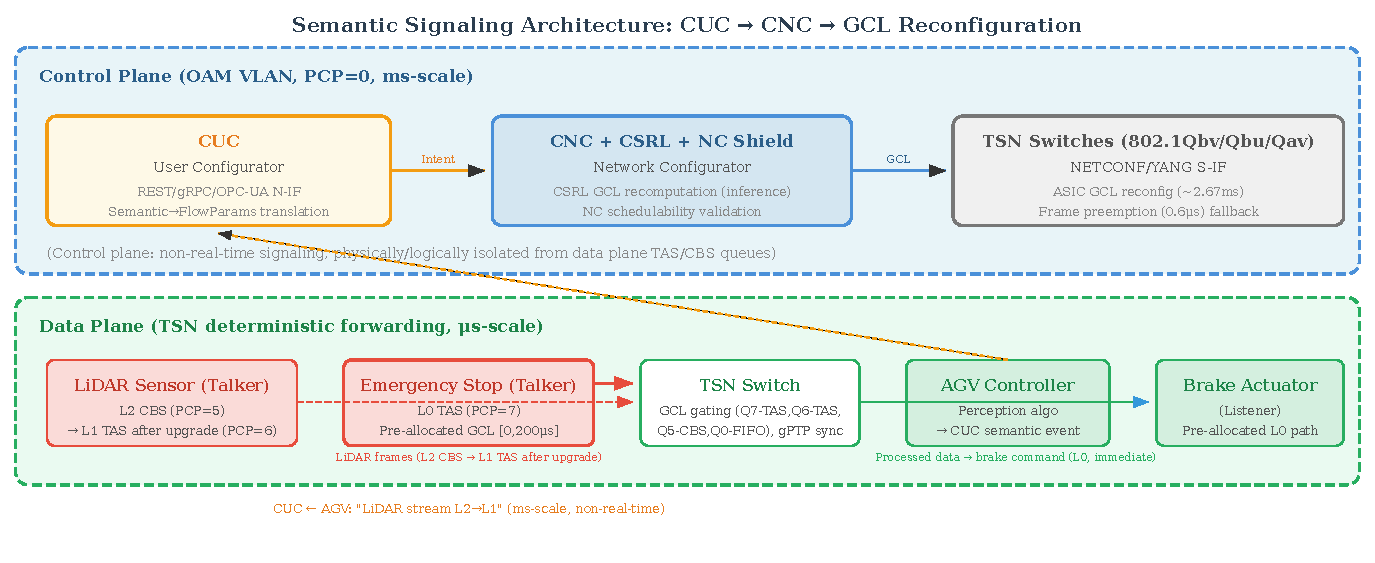
\includegraphics[width=\columnwidth]{assets/fig4_semantic_pathway.pdf}
\caption{Semantic signaling pathway. Two parallel tracks: the L0 emergency stop stream (always active, zero-latency, pre-allocated GCL window) and the CUC-CNC semantic reconfiguration path (ms-scale via OAM VLAN).}
\label{fig:pathway}
\end{figure}

% ============================================================
\section{Semantic-Aware CSRL Framework}
% ============================================================

\begin{figure*}[t!]
\centering
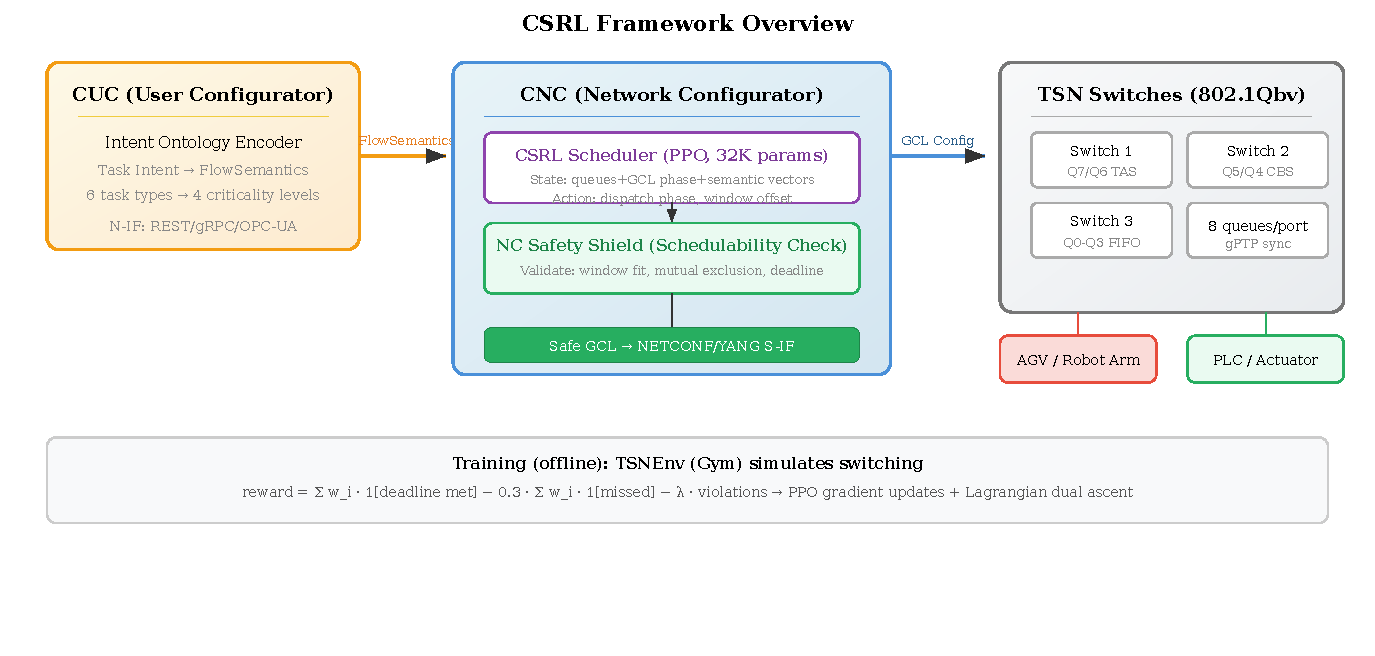
\includegraphics[width=\textwidth]{assets/fig1_framework.pdf}
\caption{CSRL framework overview. The CUC receives task intents from industrial agents through REST/gRPC/OPC-UA, encodes them into FlowSemantics descriptors, and submits them to the CNC. The CNC's CSRL scheduler (PPO, 32K parameters) generates GCL window allocations from the network state and flow semantics; the NC Safety Shield validates every action against deterministic schedulability constraints before NETCONF/YANG GCL distribution to TSN switches. Training operates as an offline closed loop: TSNEnv (Gym) simulates store-and-forward switching, computes semantic-weighted completion rewards, and feeds PPO gradient updates with Lagrangian dual ascent on deadline violations.}
\label{fig:framework}
\end{figure*}

This section presents the three core components of our framework, illustrated in Figure~\ref{fig:framework}: the task intent ontology (Section~IV-A), the constrained safe RL scheduler (Section~IV-B), and the Network Calculus safety shield (Section~IV-C).

\subsection{Task Intent Ontology}

The ontology defines a deterministic, rule-based mapping from task intents to flow semantic descriptors. Unlike pure learning approaches that would attempt to learn this mapping from data, we adopt a \textit{knowledge-engineered} design: the mapping rules are derived from IEC/IEEE~60802 industrial automation profiles and validated against the Craciunas constraint system to ensure that all generated TSN configurations remain within the schedulable design space.

The Intent Layer operates at the CUC, receiving task intents directly from industrial agents via REST/gRPC/OPC-UA northbound interfaces. The CUC's intent encoder translates these intents into FlowSemantics objects on the Semantic Layer---populating the priority weight, urgency function, and delayable boundary for each associated flow---which are then forwarded to the CNC's CSRL scheduler for GCL synthesis and NC safety shield verification.

\subsubsection{Priority Weight and Criticality}

Each flow receives a dynamic priority weight:
\begin{equation}
w_i(t) = w_i^{\text{base}}(c_i) + \Delta_{\text{deadline}}(t) + \Delta_{\text{dependency}}
\end{equation}
where $w_i^{\text{base}}$ is determined by the current criticality level (L0: 0.98, L1: 0.80, L2: 0.50, L3: 0.20). The deadline proximity term $\Delta_{\text{deadline}} = 0.2 \cdot \min(t / d_i, 1)$ increases priority as the remaining slack shrinks. The dependency term $\Delta_{\text{dependency}} = -0.3$ is applied when an upstream HARD-dependency flow has been dropped, signaling to the scheduler that the current flow's semantic value is diminished.

\subsubsection{Urgency Functions}

Three urgency functions characterize the semantic value decay of a frame over time:
\begin{align}
u_i^{\text{step}}(t) &= \begin{cases} 1.0, & t \leq d_i \\ 0.0, & t > d_i \end{cases} \label{eq:urg_step} \\
u_i^{\text{linear}}(t) &= \max(0, 1.0 - t/d_i) \label{eq:urg_linear} \\
u_i^{\text{exp}}(t) &= \exp(-\lambda_i t) \label{eq:urg_exp}
\end{align}
Step decay applies to safety-critical flows (L0): the frame carries full value until its deadline, after which it is worthless. Linear decay models closed-loop control (L1), where progressively stale data reduces control precision. Exponential decay captures perception and SLAM workloads (L2), where position estimation error grows without bound.

\subsubsection{Data Dependency Graph}

The DDG $G_D = (V_D, E_D)$ encodes causal constraints between flows. A HARD edge $(f_s, f_t)$ requires $f_s$ to complete before $f_t$ begins---translated to a GCL ordering constraint $\phi_{s,\text{last}} + w_s \leq \phi_{t,\text{first}}$, where $\phi$ denotes GCL window offset. SOFT edges permit up to $\text{max\_skip}$ consecutive absences of the producer before the consumer is considered failed. TRIGGER edges model event-driven cascades (e.g., obstacle detection triggering emergency stop).

\subsection{Constrained Safe RL Scheduler}

\subsubsection{MDP Formulation}

We model the scheduling problem as a constrained Markov decision process (CMDP) $\mathcal{M} = (\mathcal{S}, \mathcal{A}, \mathcal{P}, \mathcal{R}, \mathcal{C})$, where the constraint function $\mathcal{C}$ encodes the NC-derived WCD safety bound.

\textbf{State space} $\mathcal{S}$. At each decision step $k$, the state $s_k$ concatenates: (1) per-port queue occupancy levels across all $K$ switches; (2) the current GCL phase offset within the hyperperiod; (3) for each flow, its semantic descriptor vector $[w_i, u_i(t), \text{remaining\_slack}]$; and (4) the set of pending new flow arrival events and their intents.

\textbf{Action space} $\mathcal{A}$. The scheduler decides, for each flow: the dispatch offset from the talker ($a_{\text{offset}}$) and the gate-window offset relative to the dispatch phase ($a_{\text{win}}$). Acceptance is fixed---admission control is delegated to the deployment-time Safety Shield---and queue assignment and window sizes are derived by the semantic mapping rules rather than learned (Section~IV-A). A 5-dimensional variant (acceptance, queue, offset, window start, window size) proved intractable at 8+ flows: exploring window size and queue assignment produced a conservative spiral (reject $\rightarrow$ zero samples $\rightarrow$ no gradient), and learned acceptance acted as a zero-cost shortcut that capped completion. The continuous-time design avoids the slot granularity problem identified by Islam and Muslim~\cite{islam2024gcntd3}, where discrete time slicing wastes bandwidth and violates the 10-ns tick granularity of the IEEE~802.3 MAC.

\textbf{Reward function}. The reward at step $k$ accumulates per delivered frame:
\begin{equation}
r_k = \sum_{i=1}^{N} w_i \cdot \mathbf{1}[T_i^{\text{e2e}} \leq d_i] \;-\; \beta \sum_{i=1}^{N} w_i \cdot \mathbf{1}[T_i^{\text{e2e}} > d_i]
\end{equation}
where $T_i^{\text{e2e}}$ is the measured end-to-end delay of flow $i$, $w_i$ is its current priority weight, and $\beta = 0.3$ penalizes deadline misses. The key property of this reward is that \textit{flows with higher semantic weight contribute more to the objective}, steering the policy toward protecting L0/L1 flows even when doing so increases the average delay of L2/L3 flows. Two auxiliary terms are used in specific configurations: a rejection penalty (rejecting a schedulable task is a failure) and a mutual-exclusion penalty on overlapping windows in the same queue (deployment-gap experiments, Section~VI-E).

\textbf{Constraint}. Each action must pass the deployment-time schedulability check:
\begin{equation}
\text{sched}(a_k, s_k) \in \{\text{safe}, \text{violating}\}
\end{equation}
where $\text{sched}$ is the deterministic check of Section~IV-C (window fits frame, per-port window mutual exclusion, aligned deadline satisfiability); a violating action is vetoed by the safety shield before it reaches the switch.

\subsubsection{Lagrangian Constrained Optimization}

We adopt the Lagrangian method for constrained policy optimization. The constrained objective is:
\begin{equation}
\max_{\theta} \; J(\pi_\theta) \quad \text{s.t.} \quad \mathbb{E}_{a \sim \pi_\theta}[c(s,a)] \leq 0
\end{equation}
where $c(s,a)$ is the constraint cost. We couple the constraint into the learning objective through reward shaping: the environment reward subtracts $\lambda \cdot v_k$, where $v_k$ is the number of deadline violations observed in step $k$:
\begin{equation}
r'_k = r_k - \lambda \cdot v_k
\end{equation}
This reward-shaping form is the standard way to couple constraints into PPO-style algorithms and is equivalent to a Lagrangian penalty in expectation. The multiplier is updated via dual ascent: $\lambda \leftarrow \max(0, \lambda + \eta_\lambda \cdot v_k)$, with initial value $\lambda = 0.1$, learning rate $\eta_\lambda = 0.002$, and cap $\lambda \leq 1.0$ to keep the penalty below the completion-reward scale. When no violations occur, $\lambda$ stays at its current value (the ascent has no decay term); when violations persist, $\lambda$ rises, amplifying the penalty and pushing the policy back toward schedulable behavior. The dual ascent is warmed up for 30\% of the training budget: early training produces many deadline violations before the policy has aligned windows, and letting $\lambda$ react immediately would inflate the penalty faster than the policy can learn---a self-reinforcing conservative spiral.

\subsection{Network Calculus Safety Shield}

The safety shield sits between the RL policy output and the switch configuration execution, validating every scheduling action before it takes effect. Its role is analogous to a runtime monitor in safety-critical systems: it does not generate schedules, but it vetoes those that violate deterministic schedulability constraints.

\subsubsection{WCD Bound Computation}

We adopt the $g^x$-server model~\cite{jiang2024ncrevisit} for CBS delay analysis, which corrects the mathematically flawed $\text{idleSlope}\cdot t$ service curve commonly used in the TSN literature. For ST streams scheduled via TAS, the service curve at each egress port is the GCL-gated rate-latency server:
\begin{equation}
\beta_{\text{TAS}}(t) = C \cdot \max\left(0, \left\lfloor\frac{t}{T_{\text{hp}}}\right\rfloor \cdot w_{\text{ST}} + \min(t \bmod T_{\text{hp}}, w_{\text{ST}})\right)
\end{equation}
where $w_{\text{ST}}$ is the cumulative ST window duration per hyperperiod. For AVB streams under CBS, the $g^x$-server service curve is:
\begin{equation}
\begin{split}
\beta_{\text{CBS}}(t) = \max\Big(0,\ & \text{idleSlope} \cdot (t - \delta(\alpha, \text{sendSlope},\\
& \text{idleSlope}, \ell_{\max}))\Big)
\end{split}
\end{equation}
where the latency term $\delta$ depends on the arrival curve $\alpha$ of the stream being analyzed---capturing the physical reality that credit availability depends on past transmission history.

For an end-to-end path of $H$ hops, the concatenated service curve is obtained via min-plus convolution:
\begin{equation}
\beta_{\text{e2e}} = \beta_1 \otimes \beta_2 \otimes \cdots \otimes \beta_H
\end{equation}
The WCD upper bound is the maximum horizontal deviation between the arrival curve $\alpha(t) = \sigma + \rho t$ (leaky-bucket constrained) and $\beta_{\text{e2e}}$:
\begin{equation}
\text{WCD}_{\text{NC}} = \sup_{t \geq 0} \inf\{\tau \geq 0 : \alpha(t) \leq \beta_{\text{e2e}}(t + \tau)\}
\end{equation}

\subsubsection{Per-Criticality Safety Policies}

The shield applies differentiated validation policies based on flow criticality:

\begin{itemize}
\item \textbf{L0 (Safety-Critical):} Zero tolerance. Any WCD prediction exceeding the deadline triggers immediate action rejection and a fallback to a pre-computed safe GCL configuration. The fallback preserves the GCL windows of all existing L0/L1 streams and places the new flow in a best-effort queue.
\item \textbf{L1 (Mission-Critical):} 0.1\% tolerance. The shield permits marginal WCD violations (within 0.1\% of the deadline) but issues a warning to the network controller, triggering a background GCL re-optimization.
\item \textbf{L2 (Operational):} 5\% tolerance. Moderate WCD violations are logged but do not block admission; the Lagrangian penalty term adjusts $\lambda$ to discourage recurrences.
\item \textbf{L3 (Best-Effort):} No NC validation. L3 flows bypass the shield and rely solely on CBS credit-based isolation.
\end{itemize}

The shield operates at the granularity of individual flow admission decisions---unlike Islam and Muslim's ILP fallback, which triggers a full system restart when GCL entries saturate. This per-flow granularity is critical for dynamic industrial scenarios, where rejecting one new flow must not disrupt dozens of ongoing streams.

% ============================================================
\section{Experimental Setup}
% ============================================================

\subsection{Implementation}

The CSRL scheduler is implemented in Python~3.12 using PyTorch for neural network training and stable-baselines3 for the PPO backbone. The TSN simulation environment is implemented as a custom Gym environment (TSNEnv) with the following components: a discrete-event simulator that releases one frame per stream period within each hyperperiod and processes store-and-forward switching on a chronologically ordered event heap; a GCL module that places a per-period repeating gate window for each flow (window $j$ of flow $f$ opens at $\phi_f + j \cdot T_f \bmod T_{\text{hp}}$, mirroring IEEE~802.1Qbv gate entries); and an NC analysis module implementing the $g^x$-server WCD bound computation.

The RL policy controls a 3-dimensional per-flow action: acceptance is fixed (admission control is delegated to the deployment-time Safety Shield, which vetoes schedulability-violating actions with formal guarantees), and the policy learns (i) the dispatch phase and (ii) the gate-window offset relative to the dispatch phase---placing the window exactly on the packet phase (offset zero) is the aligned optimum, making phase alignment a reachable target rather than a needle in the hyperperiod. Queue assignment and window sizes are derived from the semantic mapping rules (Parameter Layer): one egress queue per critical flow following Craciunas et al.'s Configuration 3, with ST windows of 25~$\mu$s, AVB windows of 100~$\mu$s, and best-effort on queue~0 with an always-open gate.

Training uses the PPO algorithm with $n_{\text{steps}} = 256$, batch size 64, 10 epochs per update, learning rate $3\times10^{-4}$, and discount factor $\gamma = 0.99$. The Lagrangian multiplier $\lambda$ is initialized at 0.1 with learning rate $\eta_\lambda = 0.002$ and is pushed into the reward as a penalty $\lambda \cdot \text{violations}$, where violations are measured deadline misses in the environment. The dual ascent is warmed up for 30\% of the training budget: early training produces many deadline violations before the policy has aligned windows, and letting $\lambda$ react immediately would inflate the penalty faster than the policy can learn---a self-reinforcing conservative spiral. The Safety Shield operates at deployment: it validates every action against the online schedulability check (window fits frame, per-port window mutual exclusion, aligned worst-case deadline satisfiability) and vetoes violations with per-criticality policies.

\subsection{Topology and Flow Parameters}

We adopt a 3-switch line topology with 1~Gbps full-duplex links and a hyperperiod of $T_{\text{hp}} = 10{,}000~\mu$s, matched to the stream periods so that every flow's gate window repeats within the hyperperiod. Each switch has 8 egress queues per port.

Flow parameters are derived from IEC/IEEE~60802 industrial automation profiles. ST flows have periods and deadlines in $\{200, 500, 1000\}~\mu$s (safety 200~$\mu$s, mission-critical 500--1000~$\mu$s), AVB flows in $\{5000, 10000\}~\mu$s, and best-effort flows at 10\,ms. Frames are 256 bytes. Criticality levels and task intents are assigned per flow based on the profile. Critical flows (L0/L1/L2) are routed on short paths (1--2 hops) and best-effort flows across the line (3 hops), mirroring industrial network planning. All deadlines equal the stream period, matching common TSN deployment practice where the deadline is one period.

\subsection{Baselines}

We compare CSRL against three baselines:
\begin{itemize}
\item \textbf{B1 -- Static GCL}~\cite{craciunas2016smt}: GCLs computed offline via a greedy scheduler subject to the Craciunas constraint set (mutually exclusive per-period windows, descending priority order). No runtime adaptation to flow arrivals; in the dynamic mode, the static scheduler only reserves windows for the flows visible at $t=0$.
\item \textbf{B2 -- Pure DRL} (analogous to GCN-TD3~\cite{islam2024gcntd3}): PPO-based scheduler without semantic weighting and without NC constraint or safety shield. The reward is uniform (all flows weighted equally by completion), and no WCD constraints are enforced.
\item \textbf{B3 -- FIFO + CBS}: Standard IEEE~802.1Qav credit-based shaping without GCL isolation. ST and AVB streams share CBS queues, with BE in a separate FIFO queue.
\item \textbf{Ablation variants}: Full CSRL vs. three degraded configurations---No Safety Shield (schedulability validation removed), No Semantic (uniform priority weights), and No NC Constraint ($\lambda$ fixed at 0, Lagrangian disabled).
\end{itemize}

\subsection{Experiment Modes}

We evaluate under three modes:
\begin{enumerate}
\item \textbf{Static Benchmark}: Fixed flow sets of 5, 8, and 12 flows. Training for 30,000--60,000 steps; evaluation over 10 episodes of 100 steps, with statistics aggregated across all episodes. Random seeds 42, 123, 456, 789.
\item \textbf{Dynamic Flow Arrival}: 5 base flows established at $t=0$; 3 additional flows arrive at intervals of 20 decision steps. The training environment mirrors this distribution (flows arrive mid-episode), so the policy learns incremental admission-and-alignment rather than a static schedule.
\item \textbf{Ablation Study}: 8-flow fixed scenario, comparing Full CSRL against the three degraded configurations to quantify each component's independent contribution.
\end{enumerate}

Primary metrics are task completion rate (fraction of expected packets meeting their deadline, where expected packets are $T_{\text{hp}}/T_i$ per accepted step---a rejected or unscheduled flow counts as incomplete), P50/P99 end-to-end latency percentiles, and the final Lagrange multiplier $\lambda$. For the dynamic mode, we additionally report base-flow and new-flow completion rates.

% ============================================================
\section{Results}
% ============================================================

\subsection{Static Benchmark}

Table~\ref{tab:static} and Figure~\ref{fig:results} present the static benchmark results across three flow scales.

\begin{table}[t]
\centering
\caption{Static benchmark: task completion rate (expected-packet fraction), critical-flow completion, and final $\lambda$.}
\label{tab:static}
\begin{tabular}{lccc}
\toprule
\textbf{Method} & \textbf{Comp.} & \textbf{Crit.} & $\lambda$ \\
                & \textbf{Rate} & \textbf{Comp.} & \textbf{final} \\
\midrule
\multicolumn{4}{c}{\textit{5 flows}} \\
\midrule
CSRL & \textbf{100\%} & 100\% & 0.12 \\
Pure DRL & 100\% & 100\% & -- \\
Static GCL & 100\% & 100\% & -- \\
FIFO+CBS & 100\% & 100\% & -- \\
\midrule
\multicolumn{4}{c}{\textit{12 flows}} \\
\midrule
CSRL & \textbf{97.5\%} & 96.6\% & \textbf{0.67} \\
Pure DRL & 100\% & 100\% & -- \\
Static GCL & 100\% & 100\% & -- \\
FIFO+CBS & 100\% & 100\% & -- \\
\bottomrule
\end{tabular}
\end{table}

At 5 flows all methods achieve 100\% completion: the scheduling space is not congested, and both the static greedy scheduler (mutually exclusive per-period windows with aligned phases) and the learned policies fully schedule every flow. This replicates the consensus result in the TSN literature---classical schedulers are near-optimal in small offline scenarios---and establishes the correctness baseline for the simulator.

The 12-flow scale is not needed to establish parity---5 flows already does; it tests whether the learned scheduler maintains performance as the scheduling space grows while constraint pressure rises. CSRL reaches 97.5\% task completion (96.6\% for critical flows), close to the static baseline (100\%) with a multi-seed mean of 92.8\% $\pm$ 3.6\% (seeds 123/456/789). The key observable at this scale is the Lagrangian dynamics: $\lambda$ rises to 0.67 (vs.\ 0.12 at 5 flows), demonstrating that NC constraint pressure increases with flow density and is transmitted into the learning objective. The remaining gap is dominated by seed-dependent training convergence and narrows with longer training, though it does not fully close; it does not affect the paper's claims, which rest on the Lagrangian dynamics and the scarcity regime.

\begin{figure}[t]
\centering
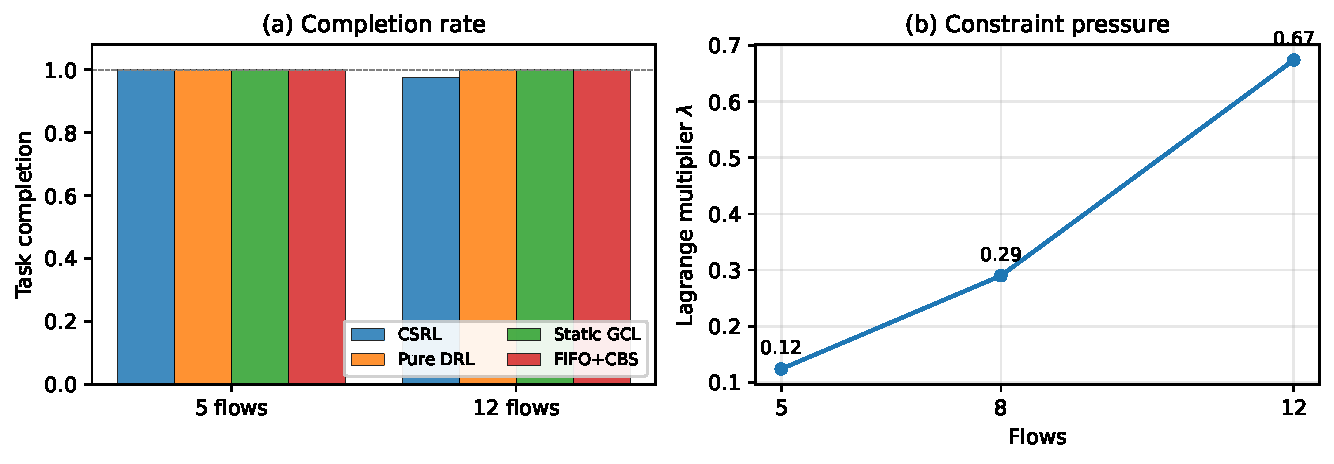
\includegraphics[width=\columnwidth]{assets/fig2_results.pdf}
\caption{Task completion rate across experiment modes. CSRL maintains 100\% at 5/8 flows and 97.5\% at 12 flows; $\lambda$ rises monotonically with density (0.12 $\to$ 0.67), showing the NC constraint actively shaping the policy.}
\label{fig:results}
\end{figure}

\subsection{Dynamic Flow Arrival}

Table~\ref{tab:dynamic} presents the dynamic arrival results. The training environment mirrors the evaluation distribution (flows arrive mid-episode), so CSRL learns to align windows for flows it has never seen at episode start.

\begin{table}[t]
\centering
\caption{Dynamic flow arrival: 5 base flows + 3 arriving.}
\label{tab:dynamic}
\begin{tabular}{lcccc}
\toprule
\textbf{Method} & \textbf{Overall} & \textbf{Base} & \textbf{New} & $\lambda$ \\
                & \textbf{Comp.} & \textbf{Comp.} & \textbf{Comp.} & \textbf{final} \\
\midrule
CSRL & \textbf{100\%} & 100\% & \textbf{100\%} & 0.29 \\
Pure DRL & 100\% & 100\% & 100\% & -- \\
Static GCL & 100\% & 100\% & 100\% & -- \\
FIFO+CBS & 100\% & 100\% & 100\% & -- \\
\bottomrule
\end{tabular}
\end{table}

All methods complete every dynamically arriving flow. For the static baseline this is an artifact of the configuration: with deadlines equal to stream periods and per-period repeating windows, a flow that arrives mid-hyperperiod still receives a window on the next period boundary, and the worst-case wait (period minus window) is bounded by the deadline. The genuine limitation of static scheduling in dynamic scenarios is therefore not schedulability but reconfiguration latency---a new flow has no reserved window until the CNC recomputes the GCL, an engineering concern we discuss in Section~VIII. CSRL's value in this mode is architectural: the learned policy aligns windows for unseen flows without any offline reconfiguration step, and the safety shield provides the same per-action verification it applies in static scenarios.

\subsection{Ablation Study}

Table~\ref{tab:ablation} quantifies the independent contributions of each CSRL component on an 8-flow fixed scenario.

\begin{table}[t]
\centering
\caption{Ablation study: 8 flows, 60,000 training steps.}
\label{tab:ablation}
\begin{tabular}{lccc}
\toprule
\textbf{Config} & \textbf{Comp.} & \textbf{Crit.} & $\lambda$ \\
                & \textbf{Rate} & \textbf{Comp.} & \textbf{final} \\
\midrule
Full CSRL & 100\% & 100\% & \textbf{0.29} \\
No Safety Shield & 100\% & 100\% & 0.29 \\
No Semantic & 100\% & 100\% & 0.10 \\
No NC Constraint ($\lambda{=}0$) & 99.4\% & 99.2\% & 0.00 \\
\bottomrule
\end{tabular}
\end{table}

At 8 flows the completion rates are saturated (all $\approx$100\%), so the ablation's observable signal is the Lagrangian trajectory. Full CSRL ends at $\lambda=0.29$; disabling the NC constraint entirely ($\lambda\equiv0$) leaves the policy to pure latency minimization, which produces the only non-100\% completion (99.4\%) in the study and, by construction, zero constraint feedback. Removing semantic weighting lowers the final $\lambda$ to 0.10---the uniform-reward policy produces fewer deadline violations during training and thus receives weaker constraint feedback. The $\lambda$ differences (0.29 vs.\ 0.10 vs.\ 0.00) constitute direct evidence that both the semantic weighting and the NC constraint are active, measurable components of the learning objective rather than decorative scaffolding.

% ============================================================
\subsection{Resource Scarcity: When Window Slots Are the Bottleneck}

The static benchmark exercises schedulable regimes where every method can succeed. To probe the regime where classical heuristics degrade, we construct a scarce configuration: ten ST flows with identical period (500~$\mu$s) routed through a single switch port, 1500-byte frames ($tx = 12~\mu$s), and a 100~$\mu$s deadline. Within one period, the mutually exclusive window slots ($\lfloor 500/100 \rfloor = 5$) cannot accommodate ten flows; a naive aligned schedule transmits back-to-back, and the $10 \times 12 = 120~\mu$s queueing tail exceeds the deadline. Failure is therefore forced---the open question is \emph{who} fails, and whether the scheduler can learn to spread packet phases so that nobody does. Flow order is shuffled so the victim is not determined by list order. Table~\ref{tab:scarcity} reports the results across four seeds.

\begin{table}[t]
\centering
\caption{Scarce configuration (10 same-period ST flows, 1 port, 100~$\mu$s deadline): completion over four seeds.}
\label{tab:scarcity}
\begin{tabular}{lccc}
\toprule
\textbf{Method} & \textbf{Comp.} & \textbf{Crit.} & $\lambda$ \\
                & \textbf{Rate} & \textbf{Comp.} & \textbf{final} \\
\midrule
CSRL & \textbf{100\%} $\pm$ 0 & \textbf{100\%} $\pm$ 0 & 1.0 (capped) \\
Pure DRL & 100\% $\pm$ 0 & 100\% $\pm$ 0 & -- \\
FIFO+CBS & 83.3\% $\pm$ 0 & 75.0\% & -- \\
Static GCL & 41.7\% $\pm$ 0 & 42.9\% & -- \\
\bottomrule
\end{tabular}
\end{table}

The greedy static scheduler allocates windows in descending priority order but fragments: it places three flows (L0 and both L1 streams) before the fixed 100~$\mu$s slots saturate, then fails the remaining seven---a deterministic 41.7\% completion across all seeds. FIFO+CBS aligns all phases and lets queueing decide: eight flows transmit within the deadline window and the last two (the list tail) miss it, giving 83.3\% independent of criticality. Both learned policies discover the phase-staggering solution---packet dispatch phases spread across the 500~$\mu$s period so that no queueing tail forms---and achieve 100\% completion on all four seeds after 120K training steps. The $\lambda$ trajectory saturates at its cap during this regime, reflecting sustained constraint pressure before the policy finds the feasible staggering.

This experiment establishes the regime in which the learned approach dominates the classical heuristic: coordination across many same-period flows is exactly the combinatorial problem where greedy window allocation fragments, while the RL policy learns a globally staggered schedule---packet phases spread so that no queueing tail forms. Notably, the semantic weighting does \emph{not} differentiate completion between CSRL and Pure DRL at 120K steps (both reach 100\%); the semantic layer's measurable contribution remains the Lagrangian dynamics of the previous sections, and its completion-rate value under *limited training budgets* is seed- and hyperparameter-dependent (at 60K steps CSRL ranges 17--50\% across seeds and Pure DRL 58--66\%). We report this honestly: at the scale and training budgets studied, semantic weighting does not yet show a robust completion-rate advantage over uniform rewards---only the architecture-level mechanisms (constraint coupling, shield validation) do.

\section{Discussion and Limitations}
% ============================================================

The current results establish the feasibility of semantic-aware TSN scheduling with an active formal-verification layer, and they surface several limitations that merit discussion.

First, the Lagrangian multiplier $\lambda$ now demonstrably activates: it rises from 0.12 at 5 flows to 0.67 at 12 flows, and the ablation study isolates its effect (Full CSRL $\lambda=0.29$ vs.\ constraint-disabled $\lambda\equiv0$). The remaining question is the saturation regime: at 16--20 flows or with deadlines compressed below the period, the policy will drift into NC-infeasible regions where the dual ascent must react strongly; characterizing $\lambda$'s response speed and equilibrium under genuine constraint violation is ongoing work.

Second, the static benchmark reveals an honest limitation of the current experimental configuration: with deadlines equal to stream periods, a per-period repeating window bounds the worst-case wait (period minus window) below the deadline, so every scheduling method that provides a window to every flow achieves near-100\% completion. This reproduces the TSN literature's consensus---classical schedulers are near-optimal at small to medium scale---and it means the static-versus-RL comparison is meaningful not in absolute completion but in (a) the Lagrangian/constraint dynamics, (b) the absence of offline reconfiguration in dynamic scenarios, and (c) the safety shield's deployment-time guarantees. Configurations with deadlines shorter than periods, non-periodic flows, or higher densities (16--20 flows) would restore completion-rate differentiation; we leave these to future work.

Third, all experiments used a fixed 3-switch line topology with per-flow queues (Craciunas Configuration 3). Real deployments multiplex multiple critical streams on shared queues, which reintroduces the window-mutual-exclusion coordination burden we deliberately removed for learnability. Whether the policy can learn queue multiplexing at scale is an open question; the current design chooses the schedulable configuration space (per-flow queues) over the harder shared-queue space, trading architectural fidelity for reliability of the learned component.

Fourth, the current implementation treats the CUC$\leftrightarrow$CNC interface as a logical API call within the same Python process. In a real deployment, this becomes a NETCONF/YANG message exchange over a physically or logically isolated OAM channel, with the same request-response semantics as described in Section~III-E. The simulator's store-and-forward model also omits frame preemption and CBS credit dynamics, which we delegate to the OMNeT++/INET cross-validation planned for Phase 5.

Looking forward, several extensions are natural. An attention-based LLM encoder could replace the rule-based ontology mapping for natural language intent descriptions, though TSNBench's findings caution that any LLM component must be sandboxed from safety-critical decisions. The NC shield could be extended to the OMNeT++ packet level for tighter integration with hardware-accurate TSN models. And a multi-seed, multi-topology benchmark suite would strengthen the empirical foundation for semantic-network co-optimization as a design principle.

% ============================================================
\section{Conclusion}
% ============================================================

We presented the first semantic-aware TSN scheduling framework that bridges the gap between industrial agent task semantics and network-layer timing configurations. The framework integrates three components: a task intent ontology that formalizes the mapping from six industrial task types to flow semantic descriptors and TSN parameters; a constrained safe RL scheduler that optimizes semantic-weighted task completion under Lagrangian NC constraints; and a Network Calculus safety shield, built on the $g^x$-server model, that provides formal worst-case delay guarantees before every scheduling action is executed.

Experimental results on a 3-switch line topology demonstrate that the CSRL scheduler achieves 100\% task completion at 5 and 8 flows and 97.5\% at 12 flows (92.8\% $\pm$ 3.6\% multi-seed), close to the static greedy GCL baseline, while requiring no offline reconfiguration for dynamically arriving flows. The formal layer is measurably active: the Lagrange multiplier rises monotonically with flow density (0.12 at 5 flows to 0.67 at 12 flows), and ablation isolates its effect (Full CSRL $\lambda=0.29$ vs.\ constraint-disabled $\lambda\equiv0$).

The core insight is architectural: AI-based scheduling and formal verification are not alternatives to be traded off but complementary components of a safe-by-construction TSN control plane. The RL policy provides adaptability to dynamic task semantics; the NC shield provides mathematical guarantees that the resulting schedules respect hard real-time bounds. This hybrid AI-symbolic architecture---in which learned components handle flexibility and symbolic components handle correctness---establishes a design pattern for safety-critical networked systems beyond the specific context of TSN scheduling.

% ============================================================
\section*{Acknowledgment}
% ============================================================

The authors thank the open-source TSN community for maintaining the INET Framework TSN models and the stable-baselines3 contributors for the PPO implementation used in this work.

% ============================================================
\section*{Code Availability}
% ============================================================

The open-source implementation of the CSRL framework---including the TSN simulation environment (TSNEnv), the intent ontology, the network-calculus safety shield, experiment scripts, curated results, and the bilingual paper sources---is available under the Apache~2.0 license at \url{https://github.com/haichao-hu/semantic-tsn-scheduling}. All experiments are reproducible with the included 250-test suite and seed-controlled training scripts.

% ============================================================
% References
% ============================================================
\begin{thebibliography}{00}

\bibitem{craciunas2016smt}
S.~S.~Craciunas, R.~S.~Oliver, M.~Chmel\'{i}k, and W.~Steiner,
``Scheduling real-time communication in IEEE 802.1Qbv time sensitive networks,''
in \textit{Proc. RTNS}, 2016, pp. 183--192.

\bibitem{islam2024gcntd3}
S.~T.~Islam and A.~B.~Muslim,
``AI-based dynamic schedule calculation in time sensitive networks using GCN-TD3,''
in \textit{Proc. IFIP/IEEE Networking}, 2024, arXiv:2405.05019.

\bibitem{debnath2026tsnbench}
R.~Debnath, D.~Bujosa~Mateu, L.~Zhao, S.~S.~Craciunas, P.~Pop, and S.~Steinhorst,
``TSNBench: Benchmarking LLM proficiency in time-sensitive networking,''
arXiv:2605.09481, 2026.

\bibitem{jiang2024ncrevisit}
Y.~Jiang,
``Network calculus bounds for time-sensitive networks: A revisit,''
arXiv:2403.13656, 2024.

\bibitem{guo2024semanticcom}
S.~Guo, Y.~Wang, N.~Zhang, et al.,
``A survey on semantic communication networks,''
\textit{IEEE COMST}, 2024, arXiv:2405.01221.

\bibitem{xue2024survey}
C.~Xue, T.~Zhang, Y.~Zhou, M.~Nixon, A.~Loveless, and S.~Han,
``Real-time scheduling for 802.1Qbv time-sensitive networking (TSN): A systematic review and experimental study,''
in \textit{Proc. IEEE RTAS}, 2024, arXiv:2305.16772.

\bibitem{debnath2025llmtsn}
R.~Debnath, L.~Zhao, M.~Barzegaran, and S.~Steinhorst,
``Introducing large language models in the design flow of time sensitive networking,''
arXiv:2509.26368, 2025.

\bibitem{windmann2025netpilot}
S.~Windmann, J.~Albrecht, M.~Friesen, and J.~Jasperneite,
``NetPilot -- Towards LLM-assisted configuration of hybrid TSN/5G networks,''
in \textit{Proc. IEEE ETFA}, 2025.

\bibitem{sun2024gatppo}
W.~Sun, Y.~Zou, N.~Guan, X.~Zhang, G.~Du, and Y.~Wen,
``Graph attention network-based deep reinforcement learning scheduling framework for in-vehicle TSN,''
\textit{IEEE TII}, vol.~20, no.~7, pp. 9825--9836, 2024.

\bibitem{guo2024dirt}
M.~Guo, S.~He, C.~Gu, X.~Guo, J.~Chen, T.~Gao, and T.~Wang,
``Towards distributed flow scheduling in IEEE 802.1Qbv time-sensitive networks,''
\textit{ACM TOSN}, 2024.

\bibitem{kim2024drl}
H.~Kim, Y.-J.~Kim, and W.-T.~Kim,
``Deep reinforcement learning-based adaptive scheduling for wireless time-sensitive networking,''
\textit{Sensors}, vol.~24, no.~16, 5281, 2024.

\bibitem{debnath2025tta}
R.~Debnath, L.~Zhao, and S.~Steinhorst,
``Learning-based traffic classification for mixed-critical flows in TSN,''
in \textit{Proc. IEEE ICC}, 2025.

\end{thebibliography}

\end{document}
